\documentclass{ximera}

\author{Bart Snapp}

\title{Working with git}

\begin{document}
\pdfOnly{\onecolumn}
\begin{abstract}
    We introduce you to \texttt{git}, and help you make changes on your own.
\end{abstract}
\maketitle

Once you've deployed our content in a GitHub codespace, you'll surely want to
change it, make it your own. Within codespace, you are running VS Code, a
full-fledged text editor. You can make changes directly there. Our files are on
the left, and are revealed by the ``pages'' icon.
Here, I've opened the folder \verb!aFirstFolder!, and then the file
\verb!aFirstActivity.tex!. I made a change in the middle of the screen.
\begin{image}
    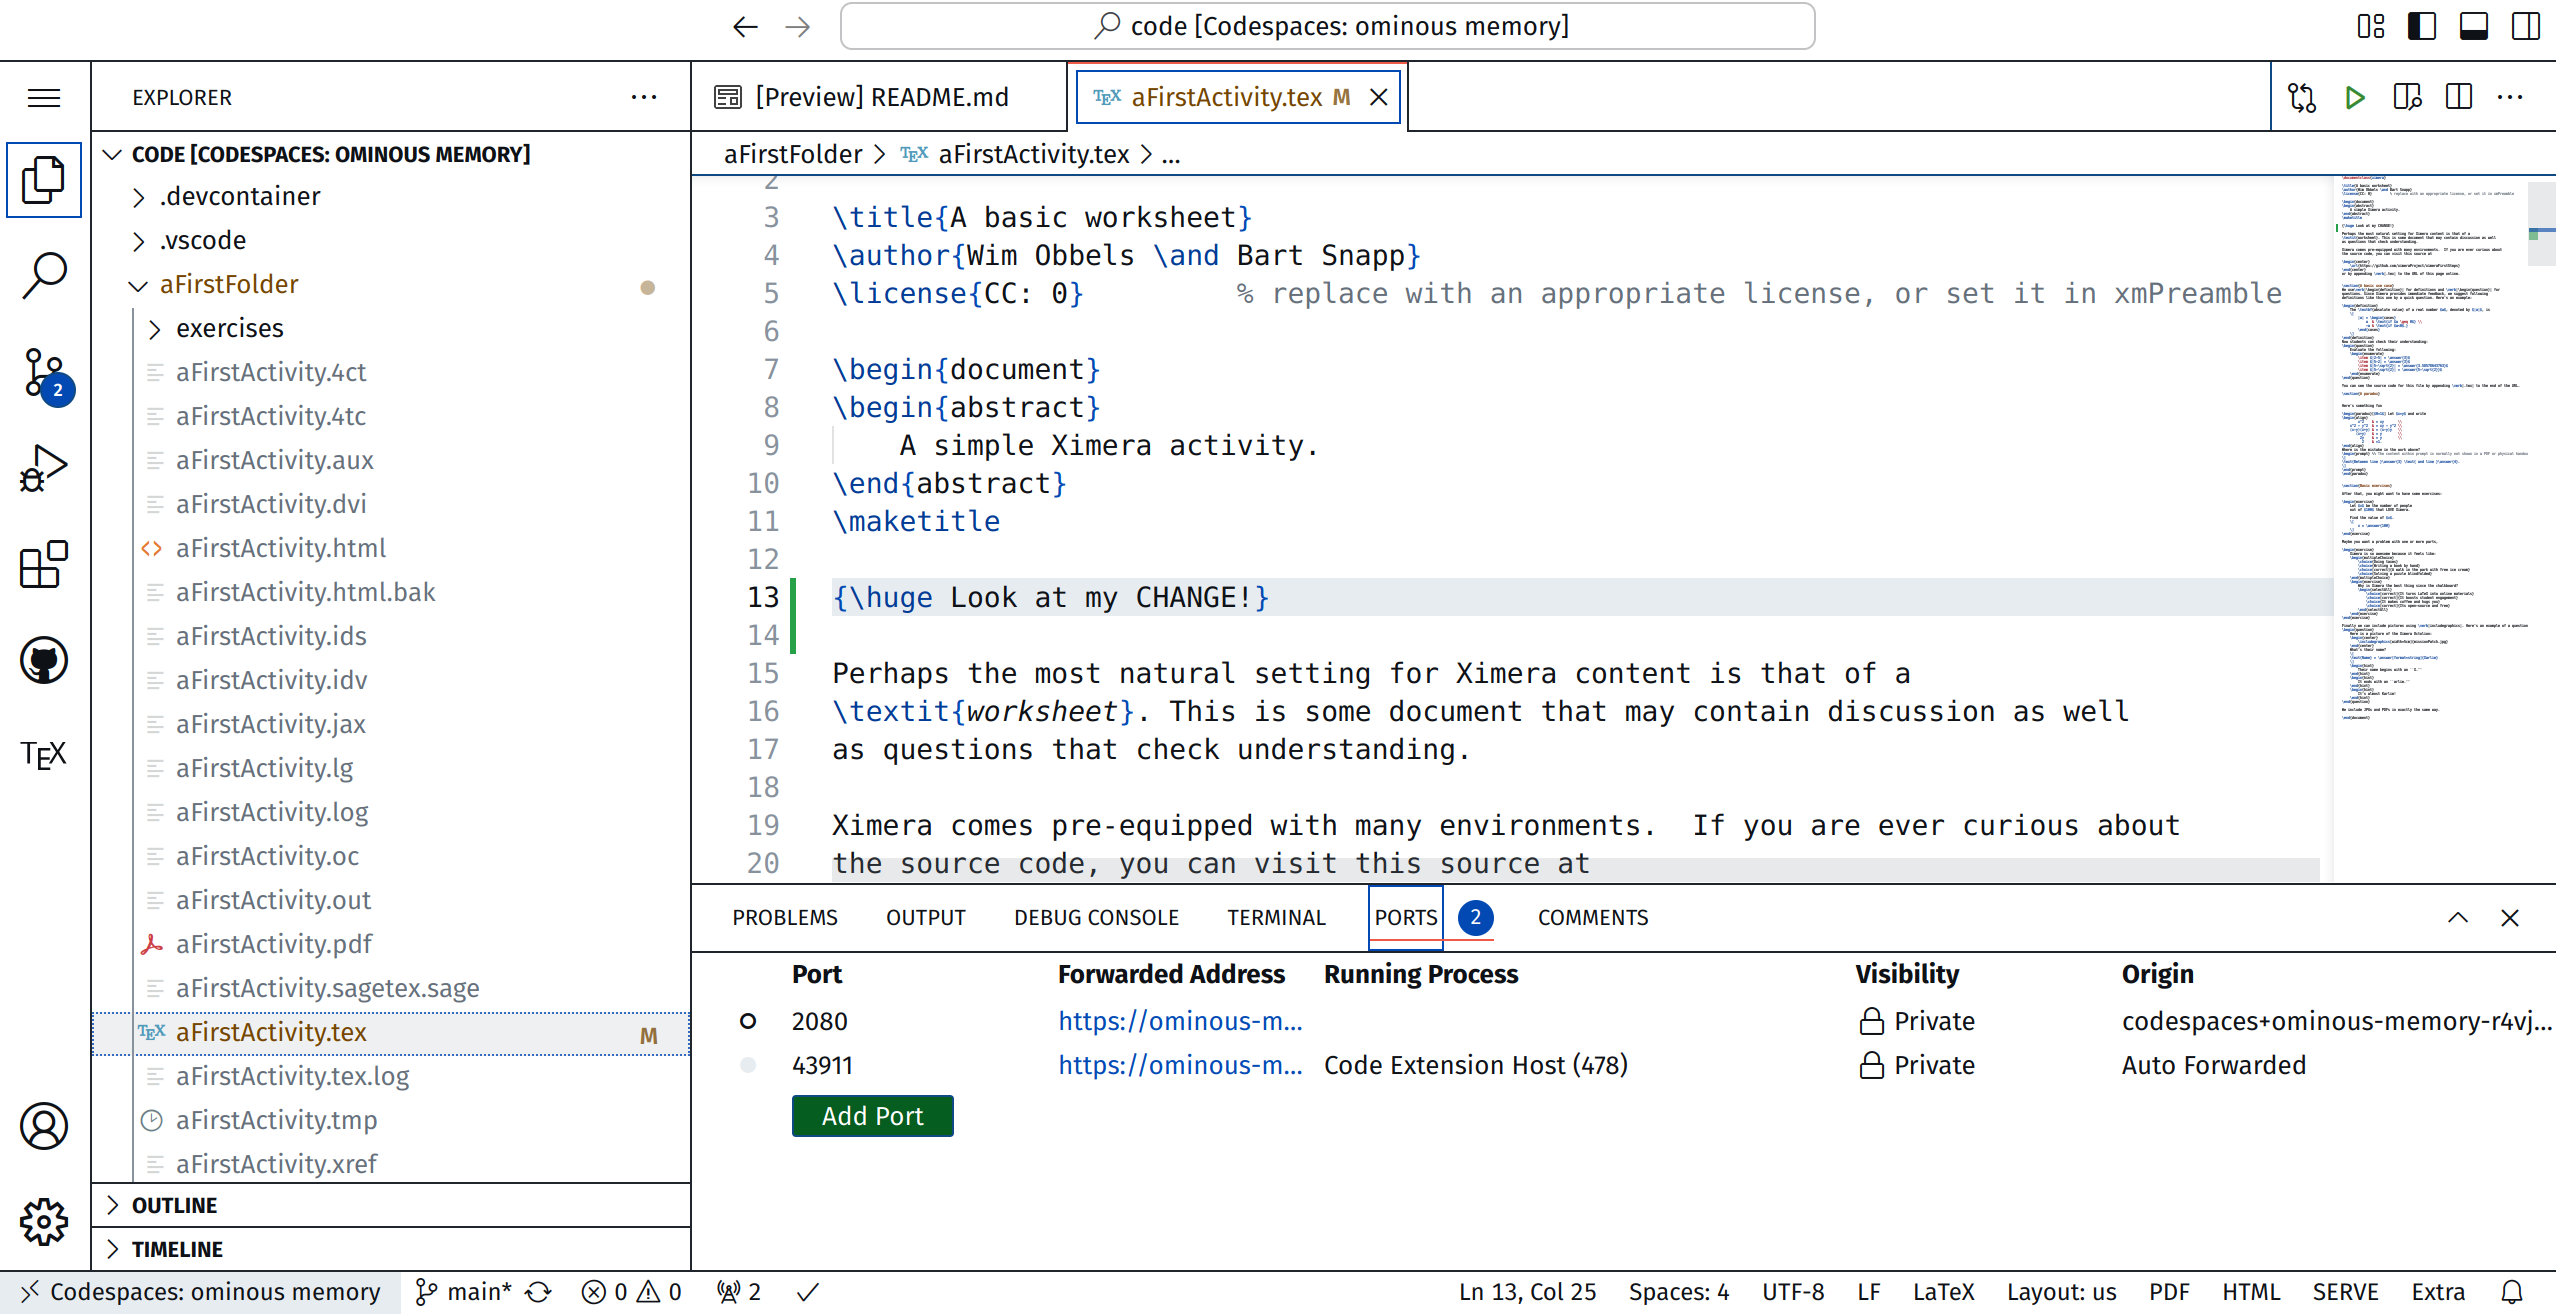
\includegraphics[width=.7\textwidth]{xfsChange}
\end{image}
At this point, you may push ``SERVE'' and see the results of your change;
however, \textbf{these changes were made only in your codespace}, a temporary
computer, lost in the cloud. To make these changes to your actual GitHub
repository, you need to ``sync'' them back.

\newpage

You start by clicking on the icon that looks like a poorly drawn ``Y'' with
lines and circles on the left. Then you click on a $+$ for every file you want
to send to your repository. You must type a message. I typed the message ``I
made a CHANGE!''
\begin{image}
    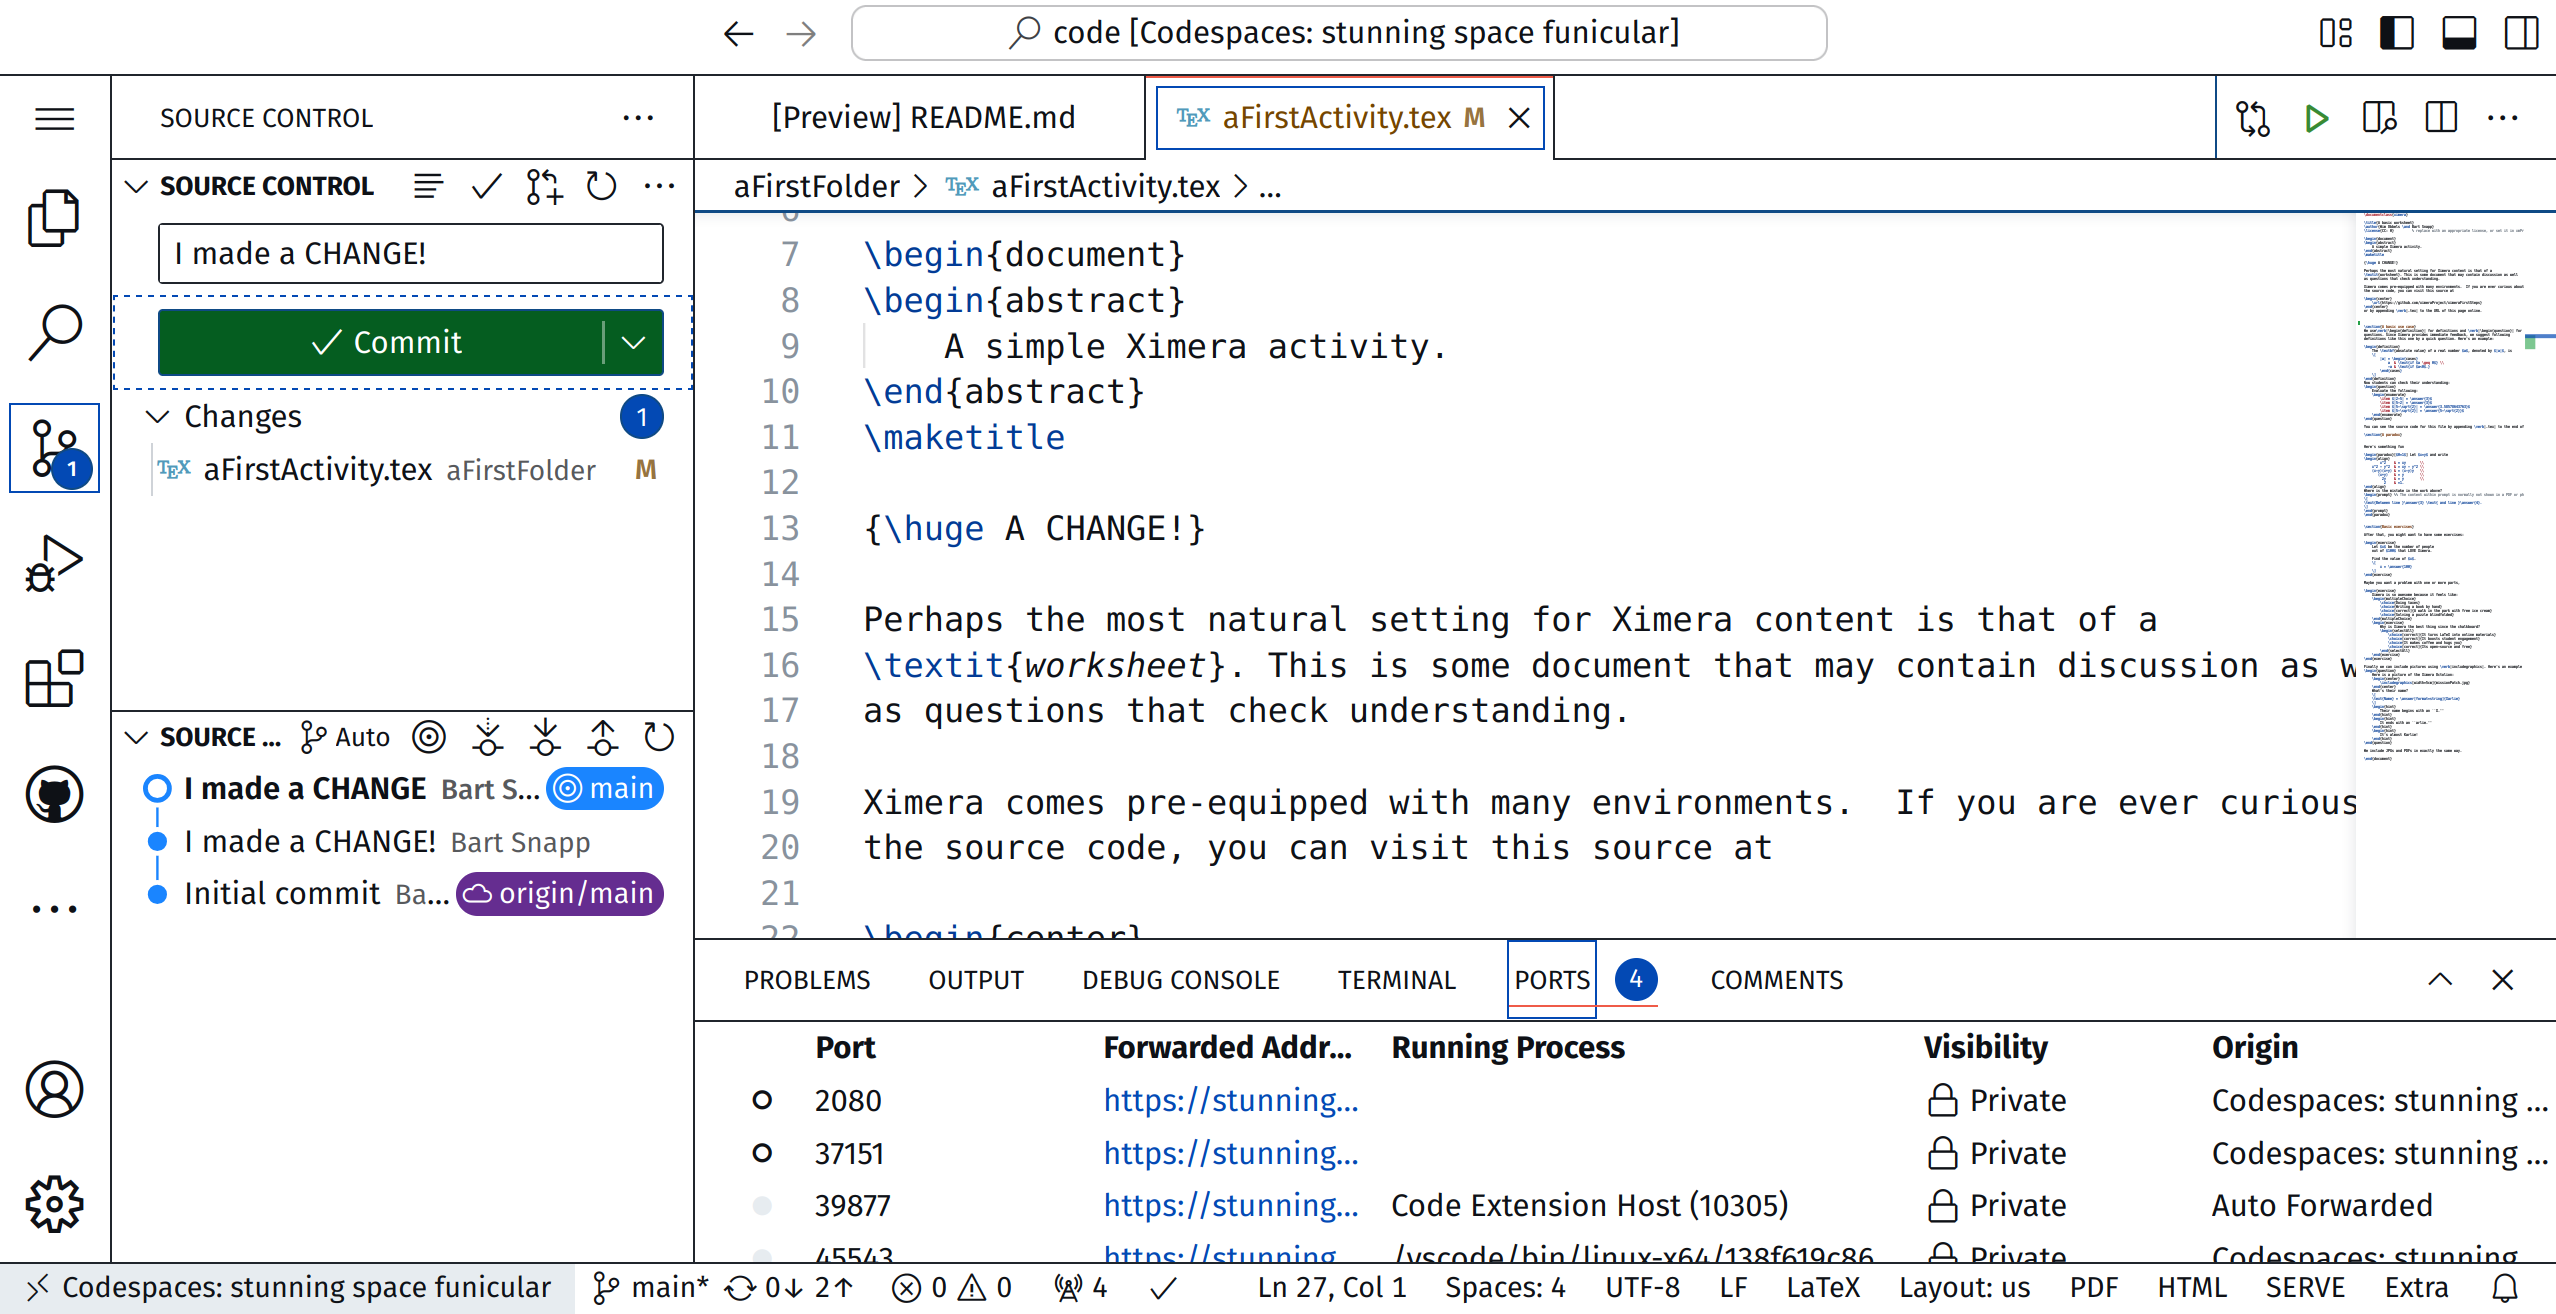
\includegraphics[width=.7\textwidth]{xfsCommitMessage}
\end{image}

\newpage

Next to the ``Commit'' button there is a carrot down. Click it, and select
``Commit and Sync.''
\begin{image}
    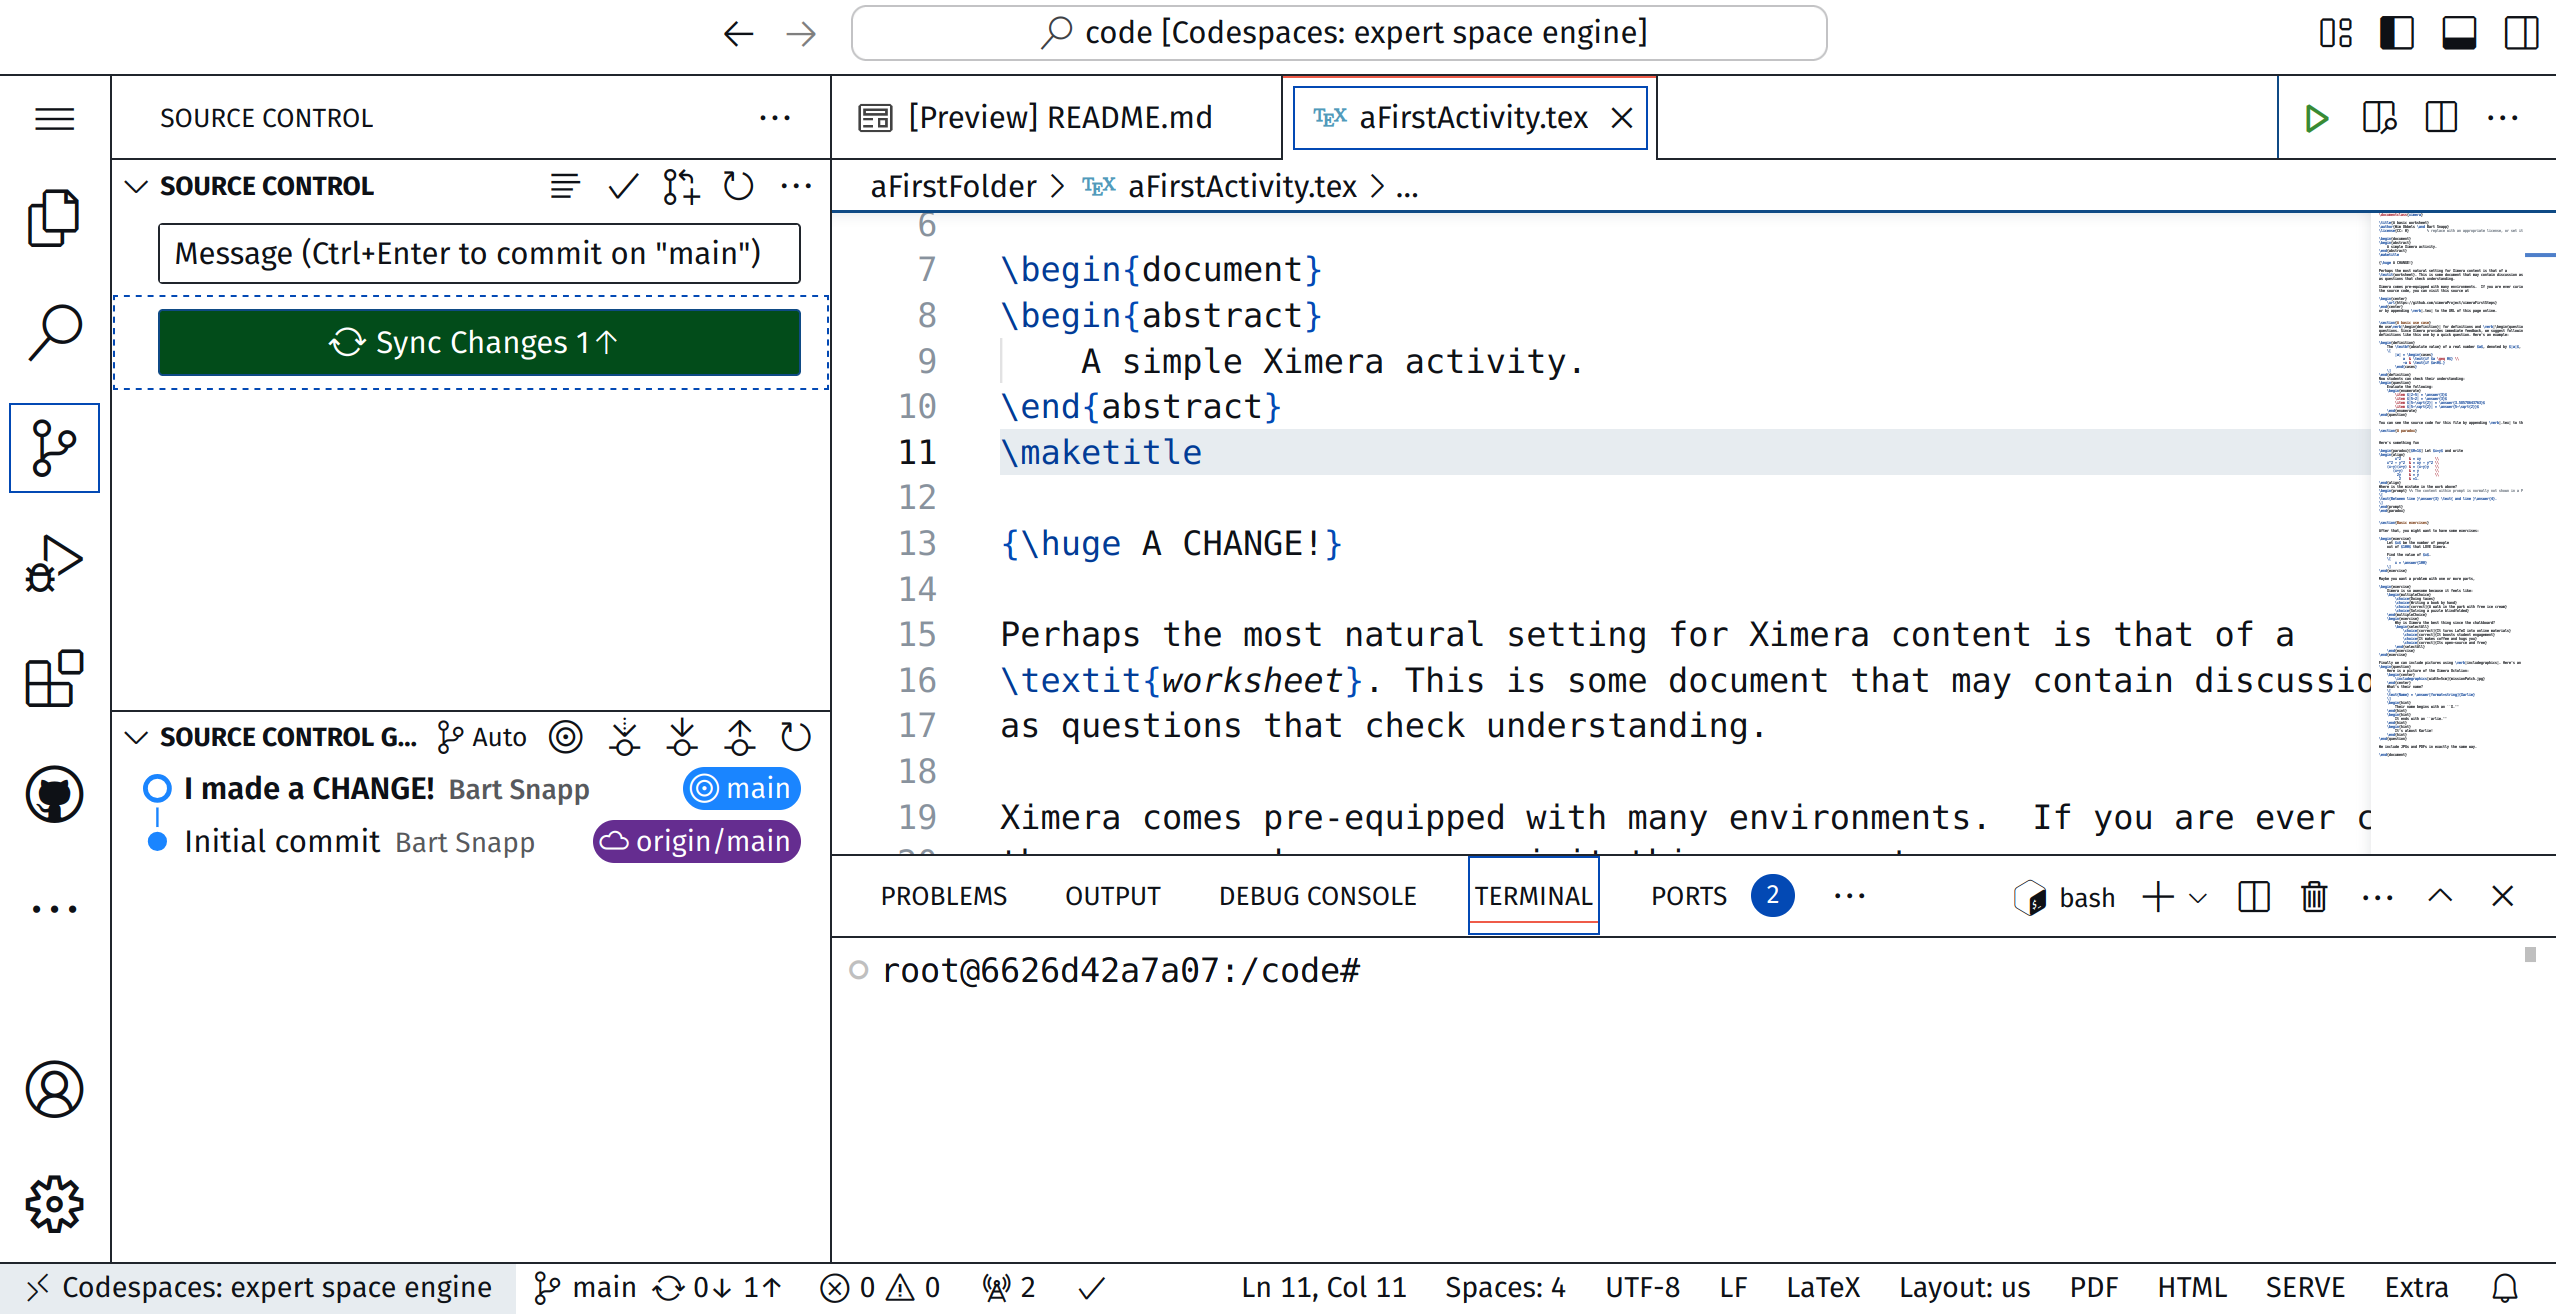
\includegraphics[width=.7\textwidth]{xfsSync}
\end{image}
Click ``Yes'' and you should be sending your changes back to your source code.

\newpage

\begin{image}
    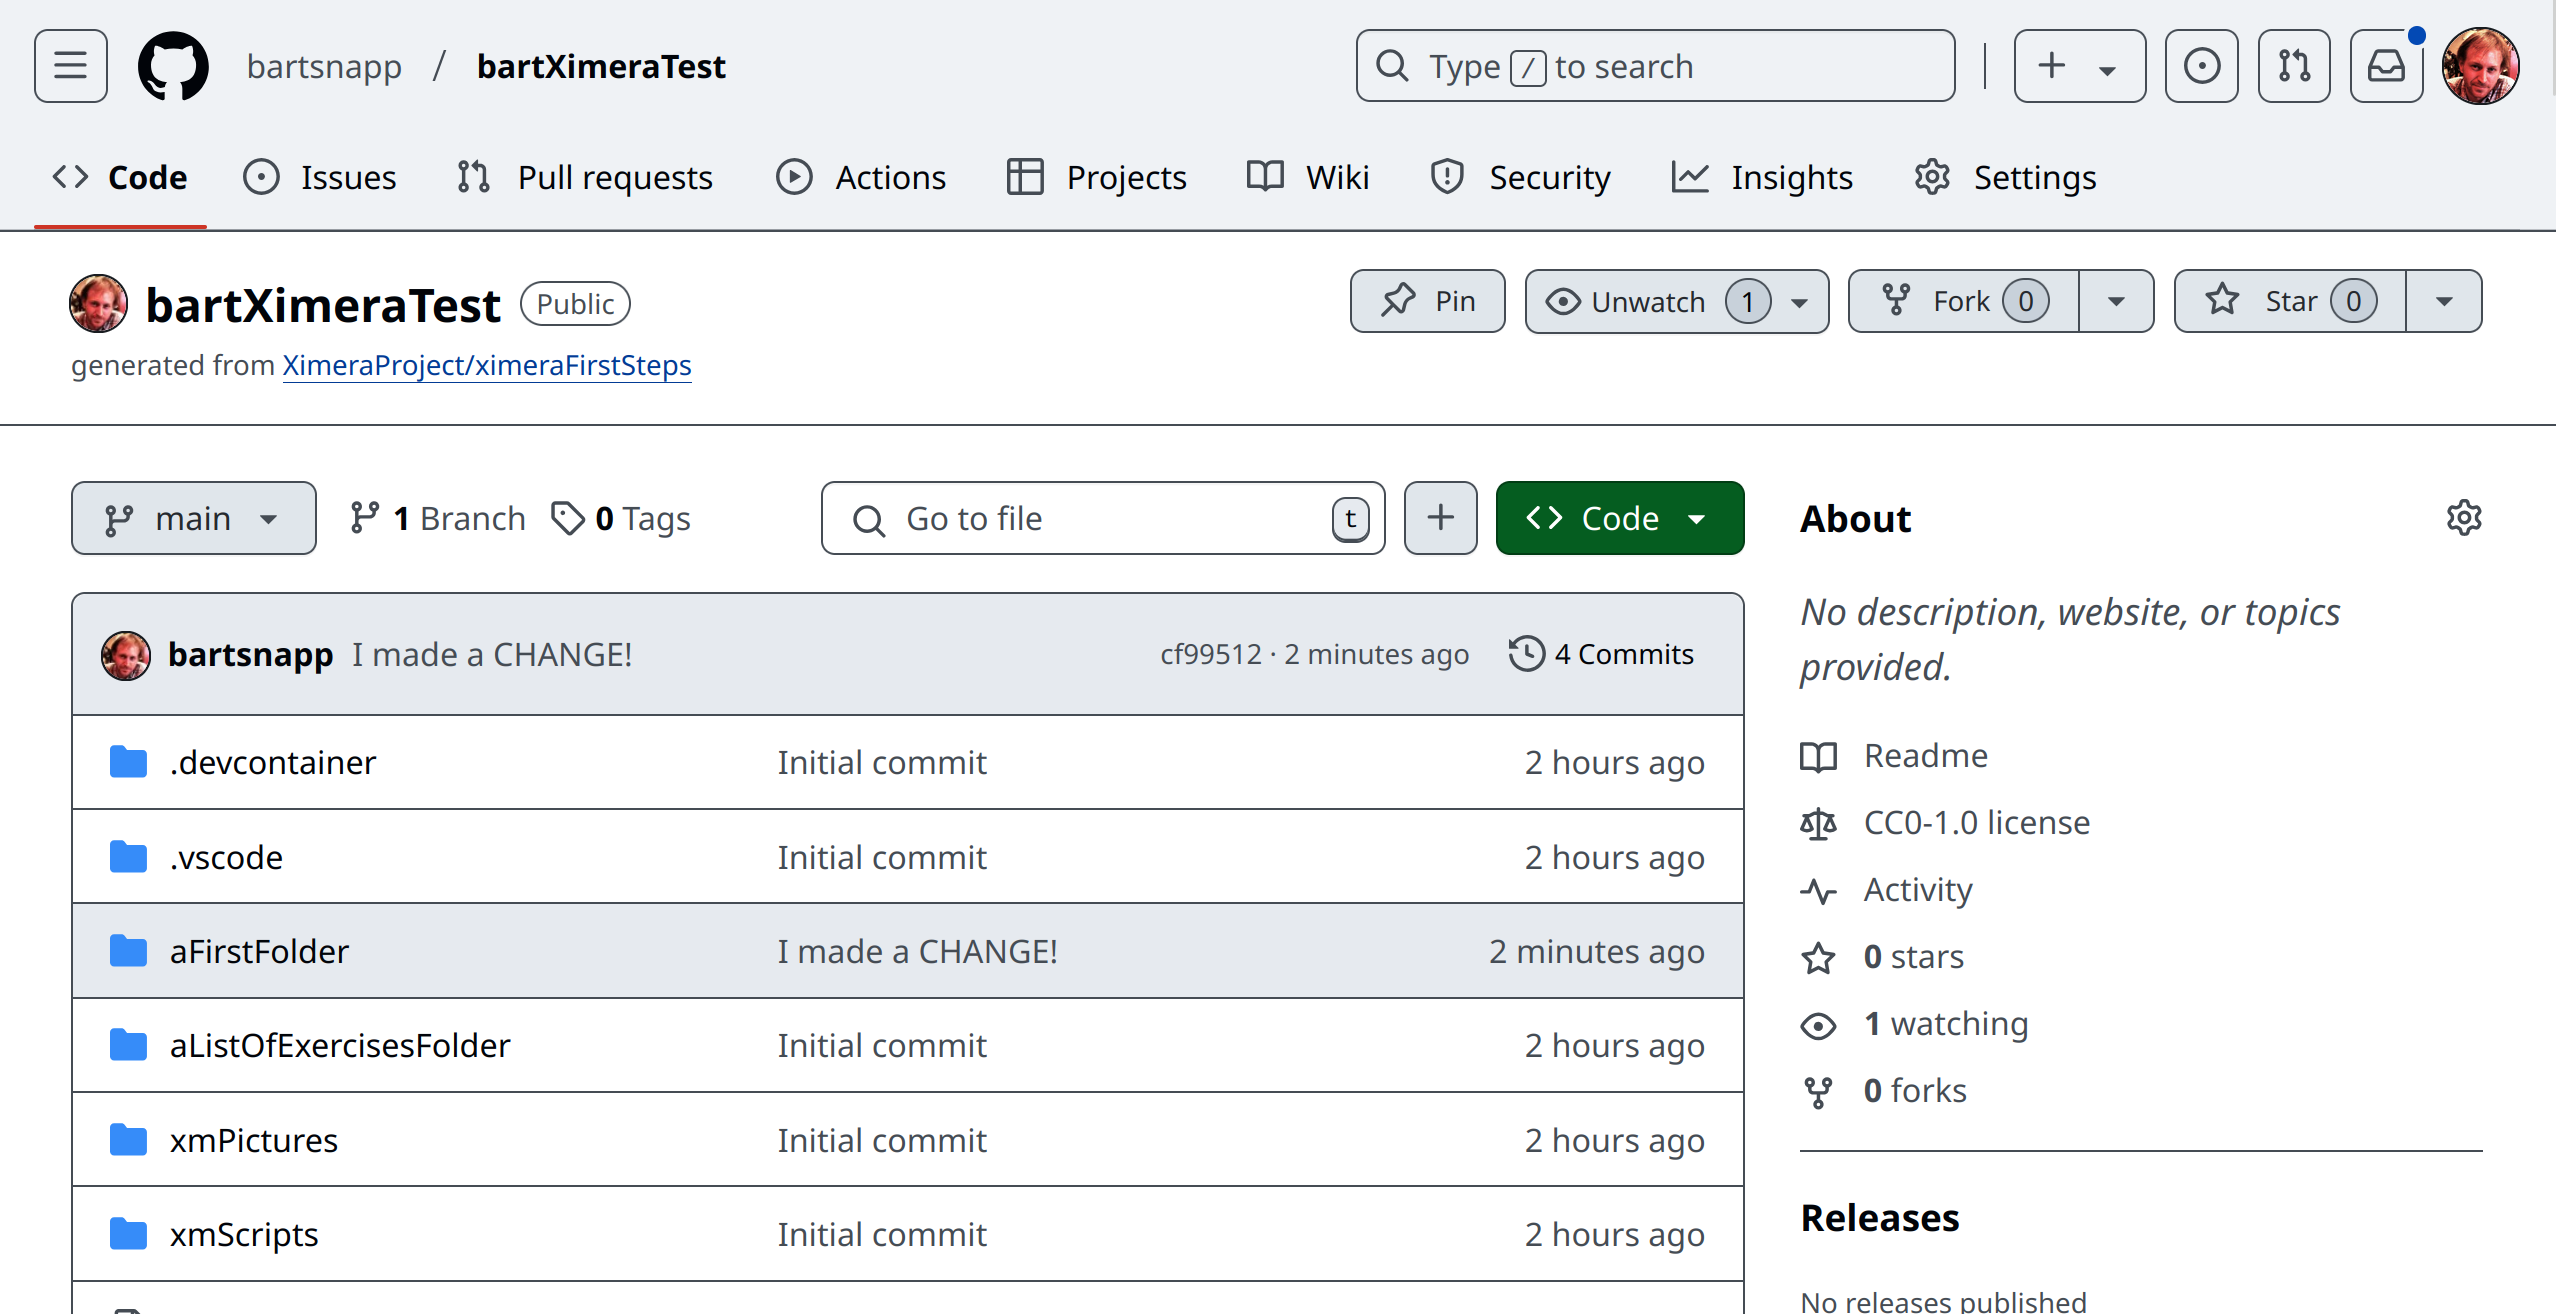
\includegraphics[width=.7\textwidth]{xfsConfirm}
\end{image}
To check that everything worked correctly, go to
\begin{center}
    \url{https://github.com/YOUR-GIT-USER-NAME/YOUR-REPO-NAME}
\end{center}
Above we see my repository, and we see that my change was indeed made.

\begin{multicols}{2}
    \section{Understanding Git Commands}

    Git is like a magical notebook that remembers every change you make to your
    project. It helps you go back in time if something breaks and lets you share
    your work with others. For this reason, it makes you do a little ``dance'' to ensure good code hygiene.

    \paragraph{Step 1: Staging Files (The ``+'' Button)}

    \textbf{What You're Doing:}
    When you click the little \textbf{``+''} next to a file, you're saying,
    \begin{quote}
        \emph{``Hey Git, this file is ready to be saved!''}
    \end{quote}

    \textbf{What Git Does:}
    This adds the file to a special list called the \textbf{``staging area.''} Only
    files in this list will be saved in the next step.

    \textbf{Command Behind the Scenes:}
\begin{verbatim}
git add <filename>
\end{verbatim}
if you want to add all updated files, do
\begin{verbatim}
git add -u
\end{verbatim}


    \textbf{Why It's Important:}
    Imagine you're painting, but you only want to save some parts of the picture
    right now. Staging lets you pick exactly which files (or changes) to save.

    \paragraph{Step 2: Committing Changes (Saving Your Work)}

    \textbf{What You're Doing:}
    After staging your files, you type a message and click \textbf{``Commit.''}
    This tells Git:
    \begin{quote}
        \emph{``Save these changes forever, and here's a note about what I did.''}
    \end{quote}

    \textbf{What Git Does:}
    Git takes a snapshot of your files and saves them with your message. It's like
    taking a picture of your work and writing a caption.

    \textbf{Command Behind the Scenes:}
    \begin{verbatim}
git commit -m 'Your commit message'
\end{verbatim}

    \textbf{Why It's Important:}
    Commits are like save points in a video game. If something goes wrong later,
    you can go back to this point and start fresh. Your notes (commit messages) are clues as to where you should go.

    \textbf{Pro Tip:}
    Always write clear commit messages, like \emph{``Fixed the login bug''} or
    \emph{``Added a new feature.''} Future-you will thank you!

    \paragraph{Step 3: Syncing with GitHub (Sending Your Work Online)}

    \textbf{What You're Doing:}
    When you click \textbf{``Commit and Sync''}, you're telling Git:
    \begin{quote}
        \emph{``Send my saved changes to the big Git notebook on GitHub.''}
    \end{quote}

    \textbf{What Git Does:}
    Git takes your saved changes and sends them to your \textbf{remote repository}
    (the one on GitHub). At the same time, it checks if there are any new changes
    from your teammates and brings them back to you.

    \textbf{Command Behind the Scenes:}
    \begin{verbatim}
git push    # Sends your changes to GitHub
git pull    # Gets changes from GitHub
\end{verbatim}

    \textbf{Why It's Important:}
    Syncing keeps everything up-to-date! You're sharing your work and making sure
    you have the latest updates from your team.

    \paragraph{The Big Idea: Git Workflow}

    Here's the step-by-step magic:
    \begin{enumerate}
        \item \textbf{Stage:} Use the ``+'' button to pick what you want to save.
              (\texttt{git add})
        \item \textbf{Commit:} Click commit and write a message to save your
              changes. (\texttt{git commit})
        \item \textbf{Sync:} Send your changes to GitHub and get updates from your
              team. (\texttt{git push}, \texttt{git pull})
    \end{enumerate}

    \paragraph{Checking Your Work}

    After syncing, go to:
    \begin{center}
        \url{https://github.com/YOUR-GIT-USER-NAME/YOUR-REPO-NAME}
    \end{center}
    You should see your changes there!
\end{multicols}
\twocolumn
\end{document}